% Created 2021-03-20 sáb 21:53
% Intended LaTeX compiler: pdflatex
\documentclass[letterpaper, 12pt]{article}
\usepackage[hidelinks]{hyperref}
\usepackage[left=2.5cm, top=2.5cm, right=2.5cm, bottom=2.5cm]{geometry}
\setcounter{secnumdepth}{0}
\usepackage[spanish, es-tabla, es-nodecimaldot]{babel}
\usepackage[utf8]{inputenc}
\usepackage{graphicx}
\usepackage{caption}
\usepackage{subcaption}
\usepackage{physics}
\usepackage{amsmath}
\usepackage{gensymb}
\usepackage{siunitx}
\usepackage{listings}
\usepackage{pdfpages}
\usepackage{cite} % referencias y bibliografía
\usepackage{babelbib}
\usepackage{enumerate}
\addto{\captionsspanish}{\renewcommand*{\listfigurename}{Índice de Figuras}}
\addto{\captionsspanish}{\renewcommand*{\contentsname}{Índice}}
\addto{\captionsspanish}{\renewcommand*{\listtablename}{Índice de Tablas}}
\pagestyle{plain}
\usepackage{eso-pic}
\usepackage[hidelinks]{hyperref}
\providecommand\phantomsection{}
\usepackage{cleveref}
\newcommand{\parg}{\par \hfill \break}
\date{\today}
\title{Diseño y análisis de Algoritmos}
\hypersetup{
 pdfauthor={Cardoso Moreno Marco Antonio},
 pdftitle={Diseño y análisis de Algoritmos},
 pdfkeywords={},
 pdfsubject={},
 pdfcreator={Emacs 27.1 (Org mode 9.5)}, 
 pdflang={Spanish}}
\begin{document}


\section{Introducción}
\label{sec:orgc085671}
\subsection{Temario}
\label{sec:orgbb0116a}
\begin{enumerate}
\item Introducción: Problemas representativos
\item Fundamentos del análisis de algotritmos
\item Grafos
\item Dividir y vencer
\item Algoritmos Voraces
\item Programación dinámica
\item Redes de flujo
\item NP e intratabilidad computacional
\item Extendiendo los límites de la tratabilidad
\item Algoritmos de aproximación
\item Búsqueda local
\item Algoritmos aleatorios
\end{enumerate}
\section{Unidad 1}
\label{sec:org3651ec9}
\subsection{Emparejamiento Estable}
\label{sec:org469d506}
Dados un conjunto de hombres y un conjunto de mujeres, ambos del mismo tamaño,
encontrar pareja a todos los hombres y todas las mujeres
\begin{itemize}
\item Monogámamente, cada persona pertenece a una sola pareja
\item Cada persona hace una lista de preferencias, en orden descendente, que incluye
a todas las personas del sexo opuesto.
\end{itemize}

Entonces:
\begin{itemize}
\item Un emparejamiento se da cuando todas las personas están a lo más en una pareja
\item Un emparejamiento perfecto se da cuando todas las personas están exactamente
en una pareja
\item Un emparejamiento es estable si es un emparejamiento perfecto y no hay
parejas inestables
\begin{itemize}
\item Una pareja es inestable si se prefieren uno al otro sobre la pareja que
tienen
\end{itemize}
\end{itemize}

El algoritmo de emparejamiento estable se inspira en \textbf{la búsqueda de pareja}.
\begin{itemize}
\item Se considera que todas las personas están libres en un principio.
\item Se tiene un grupo de mujeres y otro de hombres, ambos de la misma dimensión,
cada una de las mujeres hace un \emph{ranking} de sus preferencias sobre los
hombres, es decir, los ordena de acuerdo a cual le gusta más. Lo mismo sucede
con los hombres y sus preferencias por las mujeres.
\item Cada hombre le propone emparejarse a la \textbf{primera} mujer en su lista
\begin{itemize}
\item Ella lo acepta si está libre
\item Ella lo acepta si lo prefiere (de acuerdo a su lista de preferncias) sobre
el hombre con el que ya está
\item Ella lo rechaza y el hombre la borra de su lista y comienza de nuevo
\end{itemize}
\end{itemize}
A este algoritmo también se le conoce como \textbf{propuesta - rechazo}. El algoritmo
fue presentado por Gale-Shapley en el año 1962.
\begin{verbatim}
"Initialize each person to be free";
while ("some man is free and hasn't proposed to every woman")
{
    m = "Choose such a man m";
    w = "1st woman on m's list to whom m has not yet proposed";
    if (w isfree())
        "assign m and w to be engaged";
    else if ("w prefers m to he fiancé m'")
        "assign m and w to be engaged, and m' to be free";
    else
        "w rejects m";
}
\end{verbatim}

El análisis sobre las propiedades de este algoritmo implica, a grandes rasgos,
evaluar que éste sea correcto. Principalmente se evalúa mediante la respuesta
a ciertos aspectos:
\begin{itemize}
\item Terminación
\begin{itemize}
\item El algoritmo termina en un tiempo estimado
\item En este caso, el algoritmo termina en a lo más \(n^2\) iteraciones
\item Demostración
\begin{itemize}
\item En cada iteración en el ciclo \textbf{while}, un hombre \textbf{le propone} a una mujer
distinta
\item Tenemos \textbf{n} mujeres distintas, por tanto, cada hombre hace a lo más \textbf{n}
propuestas
\item Tenemos \textbf{n} hombres, por lo que solo puede haber a lo más \(n^2\) propuestas
\end{itemize}
\end{itemize}
\item Perfección
\begin{itemize}
\item El algoritmo obtiene un emparejamiento perfecto
\item Es decir, que todos los hombres y todas las mujeres quedan con pareja
\item Demostración (por contradicción, se basa en suponer que nuestro teorema no
es cierto)
\begin{itemize}
\item Supongamos que Carlos termina sin pareja
\item Entonces, alguna mujer quedó sin pareja, por ejemplo Celia
\item De acuerdo al algoritmo, una vez que una mujer obtiene pareja, esta ya no
es posible que vuelva a quedar libre
\item Entonces, a Celia nadie le propuso emparejarse
\item Pero, Carlos le propuso a todas las mujeres!
\end{itemize}
\end{itemize}
\item Estabilidad
\begin{itemize}
\item No hay parejas inestables
\item Demostración (por contradicción)
\begin{itemize}
\item Supongamos que Ana-Bruno es una pareja inestable, es decir, que se
prefieren uno al otro sobre la pareja que les fue asignada. O sea, que no
están juntos
\item Caso 1: Bruno nunca le propuso a Ana
\begin{itemize}
\item Esto pasa porque Bruno prefiere a su pareja asignada sobre Ana!
\end{itemize}
\item Caso 2: Bruno le propuso a Ana
\begin{itemize}
\item Ana rechazó o cambió a Bruno
\item Ana prefiere a su pareja asignada sobre Bruno!
\end{itemize}
\end{itemize}
\end{itemize}
\end{itemize}

Otras propiedades que se pueden analizar:
\begin{itemize}
\item ¿Para una instancia del problema pueden existir varios emparejamientos
estables?
\item ¿El algoritmo propuesto nos lleva a la misma solución?
\begin{itemize}
\item ¿cuál?
\item ¿de qué depende?
\end{itemize}
\end{itemize}

TARDOS - LIBRO
Proyectos en PYTHON 3.6

Boleta, Promedio, Nombre del director de tesis\ldots{}
\subsection{Problemas representativos del curso}
\label{sec:org7816927}
\subsubsection{Planificación de Tareas (Interval scheduling)}
\label{sec:org8450695}
\begin{itemize}
\item Entrada: conjunto de tareas con tiempos de inicio y final
\item Salida: el conjunto más grande de tareas compatibles.
\end{itemize}

En el ejemplo descrito en clase, se visualiza una gráfica donde se enlistan
diversas tarea, cada una con un tiempo definido para llevarse a cabo, el
objetivo del algoritmo en este caso debe ser, encontrar la solución que dé como
resultado el mayor número de tareas posibles.

Si, por ejemplo, se seleccionara la tarea \textbf{a}, solo podríamos seleccionar
después de ella a las tareas \textbf{g} u \textbf{h} (una u otra, no ambas). En la siguiente
imagen, se muestra una representación gráfica del problema, y en \textbf{azul} la
solución optima. La solución óptima es la combinación, o el set de tareas
\textbf{b}, \textbf{e} y \textbf{h}, ya que es la manera en que podemos llevar a cabo el mayor número
de tareas, sin que estas se encimen entre si.

\begin{figure}[htbp!]
\centering
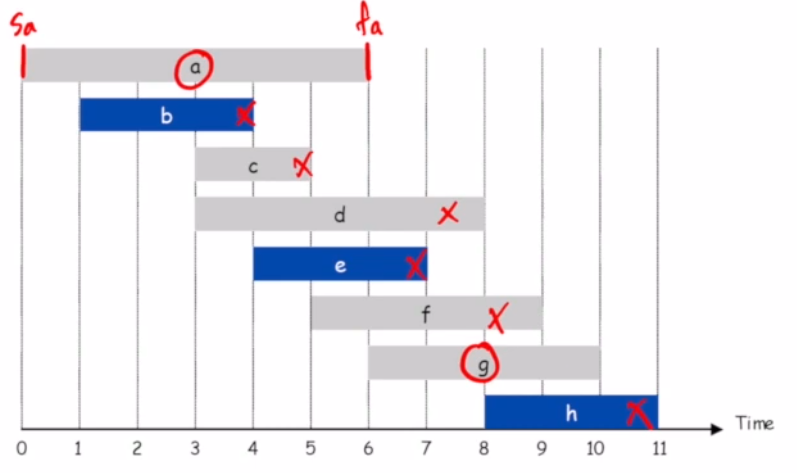
\includegraphics[keepaspectratio,width=0.5\textwidth]{./img/interval_scheduling.png}
\caption{\label{fig:interval_scheduling}Interval Scheduling. Graphical representation}
\end{figure}

Normalmente, para dar solución a este tipo de problemas, se utiliza una familia
de algoritmos conocidos comúnmente como \textbf{algoritmos voraces} o \textbf{greedy
algorithms}

\subsubsection{Planificación de tareas con pesos (Weighted Interval Scheduling)}
\label{sec:org15f2b9b}
\begin{itemize}
\item Entrada: conjunto de tarea con pesos y tiempos de inicio y final
\item Salida: el conjunto de tareas compatbiles, con el máxico peso total
\end{itemize}

Lo que se busca es escoger el set de tarea que \textbf{maximicen} la ganancia.
Manteniendo el mismo ejemplo anterior, de las tareas, y asignando un peso a
cada una de ellas, observamos que, por ejemplo, al seleccionar la tarea \textbf{a},
solo podemos escoger entre las tareas \textbf{g} y \textbf{h}. La ganancia máxima sería al
escoger las tareas \textbf{a} y \textbf{h}, lo que suma 39; sin embargo, esta no es una
solución óptima.

La solución óptima se obtiene al seleccionar las tareas \textbf{d} y \textbf{h}, ya que es la
manera en que \textbf{maximizamos} la suma de los pesos de las tareas, y que da como
resultado 49.

\begin{figure}[htbp!]
\centering
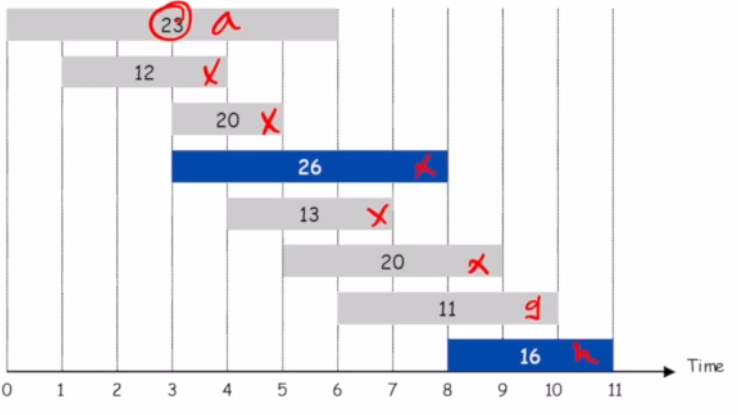
\includegraphics[keepaspectratio,width=0.5\textwidth]{./img/weighted_interval_scheduling.png}
\caption{\label{fig:weighted_interval_scheduling}Weighted Interval Scheduling. Representación gráfica}
\end{figure}

Si, por ejemplo, quisieramos utilizar la solución al problema de \textbf{Interval
Scheduling}, es decir, utilizar el set de tareas \textbf{b, e, h} tampoco obtendríamos
una solución mejor que la propuesta en color azul. En este caso, la suma de las
tres tareas es igual a 41.

Es por esto, que los greedy algorithms \textbf{NO} sirven para dar solución a
problemas de este tipo, por lo que se debe optar por otro tipo de algoritmos,
conocidos como \textbf{Algoritmos de Programación Dinámica}
\subsubsection{Emparejamiento bipartita (Bipartite Matching)}
\label{sec:orgc6cae4f}
\begin{itemize}
\item Entrada: un \textbf{grafo} bipartita
\item Salida: el emparejamiento de máxima cardinalidad
\end{itemize}

Un grafo bipartita es un grafo cuyos de nodos se puede separar en dos conjuntos,
de tal forma que no hay aristas que conecten nodos del mismo conjunto. Así como
se visualiza en la imagen. Entre letras no hay aristas que las unan entre ellas,
lo mismo pasa con los números.

\begin{figure*}
    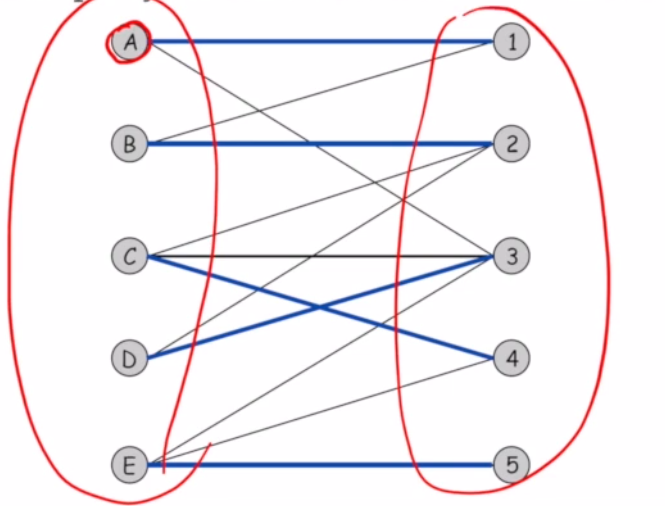
\includegraphics[width=0.7\textwidth, height=0.4\textwidth]
        {./img/bipartite_graph.png}
\end{figure*}

Si relacionamos a una letra con un número, por ejemplo la letra \textbf{A} con el
número 1, lo que evita que tanto que la letra \textbf{A} no pueda emparejarse con
ningún otro número, como que el número 1 no pueda emparejarse con ninguna otra
regla.

Entonces, el \textbf{emparejamiento bipartita} consiste en encontrar un emparejamiento
de \textbf{maxima cardinalidad}, es decir, el máximo número de parejas. No
necesariamente es igual al tamaño de cada conjunto.

Para este tipo de problemas se utilizan algoritmos de \textbf{redes de flujo} o
\textbf{augmentation}
\subsubsection{Conjunto independiente (Independent Set)}
\label{sec:org42287b0}
\begin{itemize}
\item Entrada: un grafo
\item Salida: el conjunto más grande de nodos que no están unidos por una arista
\end{itemize}

En la figura se muestra en color azul, la solución al problema del conjunto
independiente. Por otro lado, si seleccionaramos en un inicio al nodo 3, los
nodos 1, 2, 6, 7 quedan descartados y el conjunto independiente que se forma es
1, 4, 5. En cambio, el conjunto resaltado en azul (1, 4, 5, 6) es de mayor
dimensión.

\begin{figure*}
    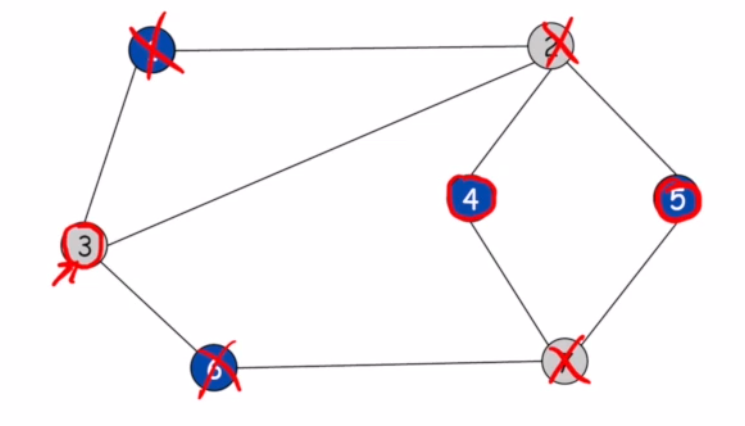
\includegraphics[width=0.7\textwidth, height=0.4\textwidth]
        {./img/independent_set.png}
\end{figure*}
\subsubsection{Tiempo de ejecución de los algoritmos}
\label{sec:orga191929}
\begin{itemize}
\item Interval Scheduling
\begin{itemize}
\item n log n -> algoritmo voraz
\end{itemize}
\item Weighted interval scheduling
\begin{itemize}
\item n log n -> programación dinámica
\end{itemize}
\item Bipartite Matching
\begin{itemize}
\item n\textsuperscript{k} -> algoritmo basado en el máximo flujo
\end{itemize}
\item Independent Set
\begin{itemize}
\item NP-completo
\end{itemize}
\end{itemize}

Un problema NP-completo, es aquel que no se puede resolver de forma optima, en
otras palabras, el problema no puede expresarse en los términos arriba
descritos, es decir, en términos de tiempo polinomial.
\section{Unidad 2 - Bases para el análisis de algoritmos}
\label{sec:orgd5e9087}
\subsection{Tratatabilidad computacional}
\label{sec:org891fef3}
\begin{itemize}
\item Eficiencia
\begin{itemize}
\item la relación entre los recursos utilizados en un proyectos y los logros que
se consiguen
\item da cuando se utilizan menos recursos para lograr un mismo objetivo
\item O, cuando se logran más objetivos con los mismos o menos recursos
\end{itemize}
\item Eficacia
\begin{itemize}
\item el nivel de consecución de metas y objetivos
\item hace referencia a nuestra capacidad para lograr lo que nos proponemos
\end{itemize}
\end{itemize}

En general, en el estudio de algoritmos, lo que nos es de \textbf{mayor interés} es la
\textbf{EFICIENCIA}.
\subsection{Tiempo de ejecución}
\label{sec:orge3512cb}
\begin{itemize}
\item Es la estimación de cuánto tiempo será necesario para que un algoritmo
encuentre la solución a un problema
\begin{itemize}
\item Este tiempo está dado en términos del tamaño de la entrada, es decir, es
una función \(f(n)\), donde \(n\) es el tamaño de la entrada para el agoritmo.
\end{itemize}
\item Se considera que todos los algoritmos son de búsqueda
\begin{itemize}
\item Búsqueda de la solución
\item Búsqueda de una propiedad
\end{itemize}
Se tiene un estado de entrada o inicial, y el algoritmo nos lleva a un estado
final o de salida. Este estado final, el \textbf{el estado que estamos buscando}, el
cual satisface los requerimientos del algoritmo.
\end{itemize}
\subsection{Análisis del peor caso}
\label{sec:orgdb80a3d}
\begin{itemize}
\item Se utiliza para obtener una cota superior del tiempo de ejecución más largo
posible para un algoritmo que tiene una entrada de tamaño N
\item Esto, en esencia, captura la \textbf{eficiencia}
\end{itemize}

En términos coloquiales, el \textbf{análisis del peor caso} es la barrera superior del
desempeño del algoritmo, se llega a éste cuando el algoritmo no es capaz de
encontrar una solución, o le toma el mayor número de pasos llegar a dicha
solución. En el caso del emparejamiento estable, el peor caso es \(n^2\), ya que
se daría cuando cada uno de los hombres se le declara a cada una de las
mujeres.

\subsection{Análisis del caso intermedio}
\label{sec:org252604e}
\begin{itemize}
\item Se busca tener una cota de tiempo de ejecución de un algoritmo con una entrada
aleatoria de tamaño N
\item Es muy difícil (si no imposible) modelar con exactitud instancias reales con
distribuciones aleatorias. En otras palabras, es muy difícil (si no imposible)
poder calcular con exactitud el caso intermedio, éste puede depender de muchos
factores.
\item Por otro lado, un algoritmo puede tener muy buenos resultados con una
distribución inicial, y pésimos resultados con otra.
\end{itemize}

En el ejemplo del emparejamiento estable, el mejor caso sería f(n) = n, que se
da cuando un hombre le propone únicamente a una mujer, para todos los hombres.
Teniendo el mejor caso (f(n) = n), y el peor caso (f(n) = n\textsuperscript{2}), sería sencillo
asumir que el caso intermedio sería f(n) = n\textsuperscript{1.5}, sin embargo, éste no será el
caso siempre.
\subsection{Fuerza Bruta}
\label{sec:orga85ad89}
NO ES ACEPTABLE, en la práctica, la búsqueda de una solución mediante \textbf{fuerza
bruta}
Video 2.1, minuto 14:10
\begin{itemize}
\item Normalmente los algoritmos de fuerza bruta tienen un tiempo de ejecución \(2^n\)
\item En el caso del emparejamiento estable, el tiempo de ejecución es \(n!\)
\end{itemize}
\subsection{Tiempo polinomial}
\label{sec:org8daa3a7}
\begin{itemize}
\item Un algoritmo funciona en tiempo polinomial si su tiempo de ejecución puede
caracterizarse como un función polinomial de la entrada \(n\). En términos
coloquiales, un algoritmo funciona en tiempo polinomial si su tiempo de
ejecución se puede escribir como un polinomio.
\item En general, se considera que los algoritmos que tienen tiempos de ejecución
polinomiales son \textbf{eficientes}
\begin{itemize}
\item con algunas excepciones, por ejemplo, polinomios con exponentes muy grandes
\end{itemize}
\end{itemize}

\textbf{agregar tabla de Tardos} que explica el profe en el video
\subsection{Órden de crecimiento asintótico}
\label{sec:orgc4f0496}
Se busca caracterizar el comportamiento del tiempo de ejecución como una función
\(f(n)\), donde \textbf{n} es el tamaño de la entrada.

Para facilitar esta búsqueda, se establece que es suficiente con caracterizar
\(f(n)\) con un órden de \emph{crecimiento asintótico}, es decir una función \(g(n)\) que
describe un límite en el comportamiento de \(f(n)\).

En términos coloquiales esto implica que, si \(f(n)\) es una función polinomial,
\(g(n)\) es un polinomio con un único término, aquel de mayor grado en \(f(n)\).
\begin{itemize}
\item Si \(g(n)\) es un \textbf{límite superior} se dice que \(f(n)\) pertenece a \(O(g(n))\).
\(O(g(n))\) representa a una familia de funciones cuyo comportamiento es acotado
por \(g(n)\).
Por ejemplo, \(O(n^2)\) representa a toda la familia de funciones \emph{cuadradas}
de \textbf{n}.
\item Si \(g(n)\) es un \textbf{límite inferior}, se dice que \(f(n)\) pertenece a \(\Omega(g(n))\)
\item Si \(g(n)\) es un \textbf{límite estrecho} para el comportamiento de \(f(n)\), se dice
que \(f(n)\) pertenece a \(\Theta(g(n))\)
\end{itemize}
\subsubsection{Límite superior (\(O\))}
\label{sec:org1c16abc}
Se dice que \(f(n)\) pertenece a \(O(g(n))\) si existen un valor inicial \(n_0\) y una
constante \emph{c}, tal que se cumpla que:
\begin{itemize}
\item \(f(n) <= c g(n)\) para toda \(n >= n_0\)
\end{itemize}

Es decir, \(c g(n)\) tiene que ser mayor que la función que describe el tiempo de
ejecución de nuestro algoritmo, \(f(n)\), a partir de un valor inicial \(n_0\).

\begin{figure*}
    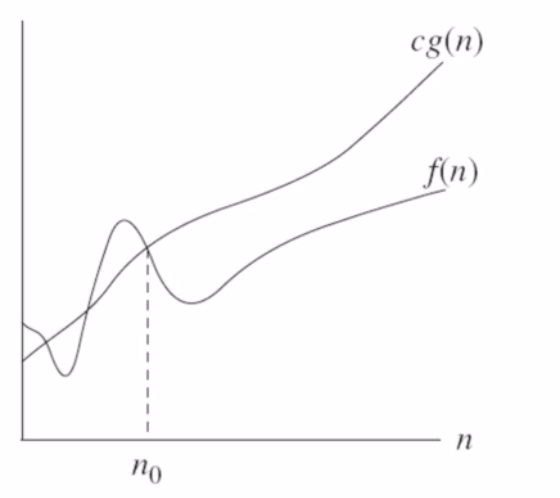
\includegraphics[widht=0.7\textwidth, height=0.4\textwidth]
        {./img/limite_superior.png}
\end{figure*}

Esta caracterización nos sirve para describir el comportamiento de nuestra
función (tiempo de ejecición) de una manera sencilla, ya que probablemente la
función \(f(n)\) tenga un comportamiento complejo.
\subsubsection{Límite inferior (\(\Omega\))}
\label{sec:org99b0851}
Lo mismo sucede para el caso del límite inferior. Decimos que \(f(n)\) pertenece a
\(\Omega(f(n))\), si existen un valor inicial \(n_0\) y una constante \emph{c}, tal que
\begin{itemize}
\item \(f(n) >= c g(n)\) para toda \(n >= n_0\)
\end{itemize}
Es decir, podemos caracterizar el límite inferior de \(f(n)\), de manera más
sencilla, mediante el comportamiento de \(\Omega(g(n))\) si el valor de \(f(n)\) es
mayor en todo momento que el valor de \(c g(n)\) a partir de un valor inicial
\(n_0\).

\begin{figure*}
    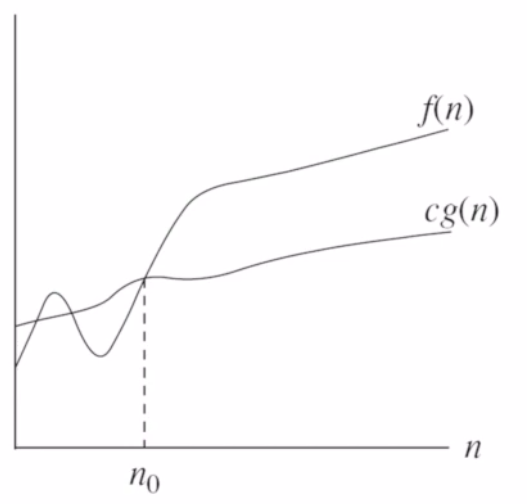
\includegraphics[width=0.7\textwidth, height=0.4\textwidth]
        {./img/limite_inferior.png}
\end{figure*}
\subsubsection{Límite estrecho (\(\Theta\))}
\label{sec:orgc6ce78c}
Se dice que \(f(n)\) pertenece a \(\Theta(g(n))\) si existen las constantes \(c_1\) y
\(c_2\), además de un valor inicial \(n_0\) para los cuales se cumple que:
\begin{itemize}
\item \(c_1 g(n) <= f(n) <= c_2 g(n)\) para toda \(n >= n_0\)
\end{itemize}

\begin{figure*}
    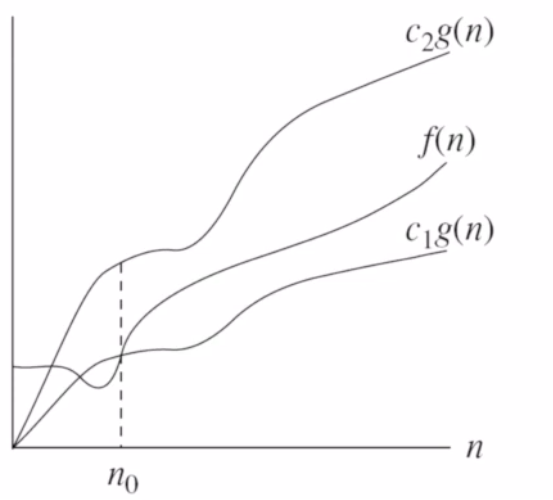
\includegraphics[width=0.5\textwidth, keepaspectratio]
        {./img/limite_estrecho.png}
\end{figure*}
\subsubsection{Propiedades}
\label{sec:org4211e98}
\begin{itemize}
\item Transitividad
\begin{itemize}
\item Si \(f(n)\) es \(O(g(n))\) y \(g(n)\) es \(O(h(n))\) entonces \(f(n)\) es \(O(h(n))\)
\item Si \(f(n)\) es \(\Omega(g(n))\) y \(g(n)\) es \(\Omega(h(n))\) entonces \(f(n)\) es
\(\Omega(h(n))\)
\item Si \(f(n)\) es \(\Theta(g(n))\) y \(g(n)\) es \(\Theta(h(n))\) entonces \(f(n)\) es
\(\Theta(h(n))\)
\end{itemize}
\item Reflexividad
\item Simetría
\item Simetría transpuesta
\item Aditividad
\end{itemize}

\subsubsection{Demostraciones}
\label{sec:org5d2b0c2}
\begin{itemize}
\item implicacion: entonces (==>)
\item si y solo si (\texttt{=>, <=}), si uno es cierto, el otro tambien es cierto, se debe
hacer la demostración en ambos sentidos
TAREA EN PDF, GENERADO EN LATEX
\end{itemize}
\subsection{Compilación de tiempos de ejecución comunes}
\label{sec:org6d5e258}
\subsubsection{Tiempo constante \emph{O(1)} o \(O(n^0)\)}
\label{sec:org777ad5a}
\begin{itemize}
\item El tiempo de ejecución \textbf{no depende} del tamaño de la entrada
\item Ejemplos:
\begin{itemize}
\item Dado un arreglo ordenado d \emph{N} elementros, devolver el elemento más grande
\item Dado un arreglo de \emph{N} elementos, devolver los primeros \emph{K} elementos
\end{itemize}
\end{itemize}
\subsubsection{Tiempo sublineal \(O(\log n)\)}
\label{sec:org967429f}
\begin{itemize}
\item El tiempo de ejecución es muy eficiente ya que crece muy poco con respecto al
tamaño de la entrada.
\item Ejemplo:
\begin{itemize}
\item \emph{Binary search}: Dado un arreglo ordenado de elementos, realizar la búsqueda
de un elemento en particular. El siguiente bloque de código muestra un
código de \emph{binary search} en lenguaje \emph{python}.
\end{itemize}
\end{itemize}
\begin{verbatim}
 1  import math
 2  
 3  def binary_search_iter(A, x, left, right):
 4      """
 5      A = array of numbers
 6      x = number to search for
 7      left, right = begining and end of array, respectively
 8      """
 9      while (left <= right):
10          middle = (left + right) / 2 # O(1) no depende del tamaño N
11          if A[middle] == x:          # O(1) no depende del tamaño N
12              return middle           # O(1) no depende del tamaño N
13          elif A[middle] > x:         # O(1) no depende del tamaño N
14              right = middle - 1      # O(1) no depende del tamaño N
15          else:
16              left = middle + 1       # O(1) no depende del tamaño N
17  
18      return -1                       # O(1) no depende del tamaño N
\end{verbatim}

El código se puede analizar mediante un técnica conocida como \textbf{ley de sumas}. Se
observa que todas las operaciones dentro del ciclo \texttt{while} son \(O(1)\) (no
depende de la entrada), por lo que la ejecución del ciclo es en tiempo
constante. Sin embargo, el número de veces que se ejecuta el ciclo \texttt{while} es
variable, ya que en cada iteración (en las líneas 14 y 16) se desplaza alguno de
los pivotes a la mitad del espacio de búsqueda, por lo que en cada iteración
se reduce a la mitad el espacio de búsqueda (inicialmente el array completo).
\begin{itemize}
\item \(N\), \(\frac{N}{2}\), \(\frac{N}{4}\), \(\frac{N}{8}\), \(\cdots\), \(1\)
\end{itemize}

La función logarítmica nos indica cuántas veces podemos dividir un número entre
la base del logaritmo, en el caso de la \emph{binary search} el número de veces que
se ejecuta el ciclo \texttt{while} es \(\log_2(n)\). Si observamos que tenemos dentro de
éste seis operaciones \(O(1)\), y que el \texttt{return} es de igual manera \(O(1)\),
tenemos que:
$$
f(n) = 6 \log_2(n) + 1 \therefore f(n) \in O(log(n))
$$
\subsubsection{Tiempo lineal \emph{O(n)}}
\label{sec:orgd0d4b45}
\begin{itemize}
\item El tiempo de ejecución es, a lo más, un factor de tiempo constante por el
tamaño de la entrada.
\item Ejemplo:
\begin{itemize}
\item calcular el máximo de un conjunto de números
\(A = \{a_1, a_2, \cdots, a_n\}\). El siguiente bloque de código muestra el
algoritmo.
\end{itemize}
\end{itemize}
\begin{verbatim}
1  max = a[0]              # O(1)
2  for i in range(1, n):
3      if a[i] > max:      # O(1)
4          max = a[i]      # O(1)
\end{verbatim}

Se observa que el ciclo \texttt{for} se ejecuta \(n-1\) veces, y que dentro de él hay dos
operaciones de tiempo lineal. Además, la primer asignación \texttt{max = a[0]} tambien
se ejecuta en tiempo lineal, lo que nos da como resultado:
$$
    f(n) = 2 \left(n -1\right) + 1 = 2n - 1 \therefore f(n) \in O(n)
    $$
\begin{itemize}
\item Combinar dos conjuntos de números ordenados \(A = \{a_1, a_2, \cdots, a_n\}\) y
\(B = \{b_1, b_2, \cdots, b_m\}\). A este algoritmo se le conoce como \emph{merge
sort}, la figura \ref{fig:merge_sort_lineal} muestra un esquema gráfico del algoritmo

\begin{figure}[htbp!]
\centering
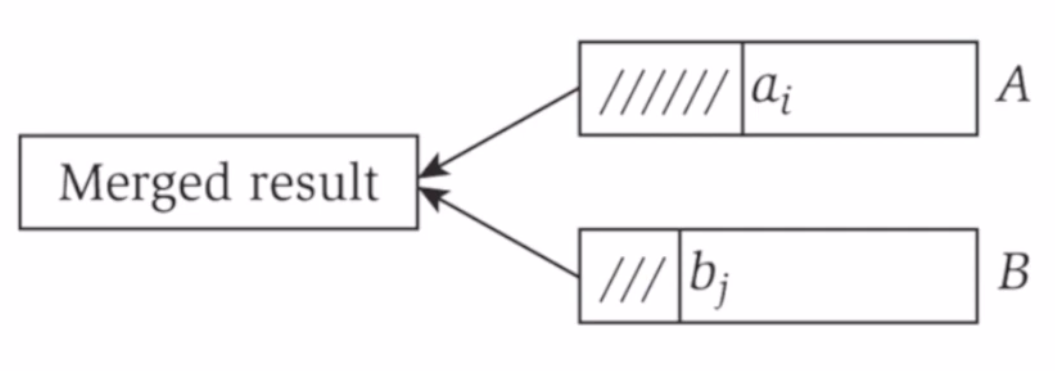
\includegraphics[keepaspectratio,width=0.4\textwidth]{./img/merge_sort_lineal.png}
\caption{\label{fig:merge_sort_lineal}Esquema gráfico del algoritmo \emph{merge sort}}
\end{figure}

El algoritmo se puede expresar como:
\begin{verbatim}
i = 0;
j = 0;

while (i < len_a && j < len_b)
{
    if (a[i] < b[j])
    {
        merged[i + j] = a[i];
        i++;
    }
        else
    {
        merged[i + j] = b[j];
        j++;
    }
}

if (i < len_a)
    // append rest of a to merged
else if (j < len_b)
    // append rest of b to merged

return (merged);
\end{verbatim}

El algoritmo comienza con los arrays \emph{a} y \emph{b}, utilizando los índices \emph{i} y
\emph{j} para avanzar sobre \emph{a} y \emph{b} respectivamente. En cada iteración del loop
\texttt{while} comparamos los elementos de cada array, el que sea mayor es agregado
al arreglo \texttt{merged}, y se incrementa el índice correspondiente. Este proceso
continúa hasta que se haya acabado con alguno de los arrays \emph{a} y \emph{b}.

Las asignaciones que anteceden al ciclo \texttt{while} son tiempo constante
\(f(n) = 1\), y son dos de ellas. Dentro del ciclo \texttt{while}, las tareas de
comparación, asignar los elementos al array \texttt{merged} y el incremento, son
tres operaciones \(f(n) = 1\), como el condicional \texttt{if} es excluyente, no
importa qué rama es la que se toma, el valor es 3 de igual modo. El ciclo
\texttt{while}, por su lado, se ejecuta \(2n - 1\) veces en el peor de los casos,
si es que siempre se intercalan los valores de \emph{a} y \emph{b}. Y por último,
agregar el resto de una de las dos listas, tiene un costo, en el peor caso,
de \(n\), que se da si todos los elementos de una lista, son menores al
primer elemento de la otra lista, por lo que se agregaría la lista menor,
entera, primero y posteriormente la segunda, completa.

El coste total entonces es:
$$
    f(n) = 2 + (2n - 1) + n = 3n - 1 \Rightarrow f(n) \in O(n)
    $$

La demostración formal se lleva a cabo de la siguiente manera:
\begin{itemize}
\item El conjunto \emph{A} se vacía:
\begin{itemize}
\item En el mejor caso, en \emph{n} iteraciones
\begin{itemize}
\item Todos los elementos del conjunto \emph{A} son menores que el primer
elemento del conjunto \emph{B}
\end{itemize}
\item En el peor de los casos, en \(2n\) iteraciones
\begin{itemize}
\item El primer elemento de \emph{A} es mayor que todos los elementos de \emph{B}
\end{itemize}
\end{itemize}
\item El conjunto \emph{B} se vacía:
\begin{itemize}
\item En el mejor caso, en \(2n\) iteraciones
\begin{itemize}
\item Todos los elementos del conjunto \emph{A} son menores que el primer
elemento del conjunto \emph{B}
\end{itemize}
\item En el peor de los casos, en \(2n\) iteraciones
\begin{itemize}
\item El primer elemento de \emph{A} es mayor que todos los elementos de \emph{B}
\end{itemize}
\end{itemize}
\end{itemize}
\end{itemize}
\subsubsection{Tiempo logarítmico \(O(n \log n)\)}
\label{sec:org5ad5361}
Surge en los algoritmos \emph{divide and conquer}
\begin{itemize}
\item Ordenar un conjunto \emph{n} de números
\begin{itemize}
\item Mergesort
\item Heapsort
\end{itemize}
\item Encontrar el camino, en un grafo, más corto desde un nodo hacia todos los
demás nodos
\end{itemize}

La figura \ref{fig:merge_sort} muestra un esquema gráfico del algoritmo \emph{mergesort}.
En esta se observa que se comienza haciendo particiones del array que se va a
ordenar, este proceso es recursivo hasta que nos quedamos con arrays con un solo
elemento, una vez que se llega a este punto, comenzamos a regresar hacia el
array original pero esta vez ordenando los elementos de cada uno de los arrays.
Se considera que un arreglo de talla uno está ordenado, se hace el \emph{merge}
(el algoritmo descrito en el tiempo de ejecución lineal)  para obtener arrays de
talla dos, los cuales \textbf{ya están ordenados}, y se continúa este proceso; ahora se
mezclan arrays de talla dos para obtener arrays ordenados de talla 4, y así
sucesivamente.

\begin{figure}[htbp!]
\centering
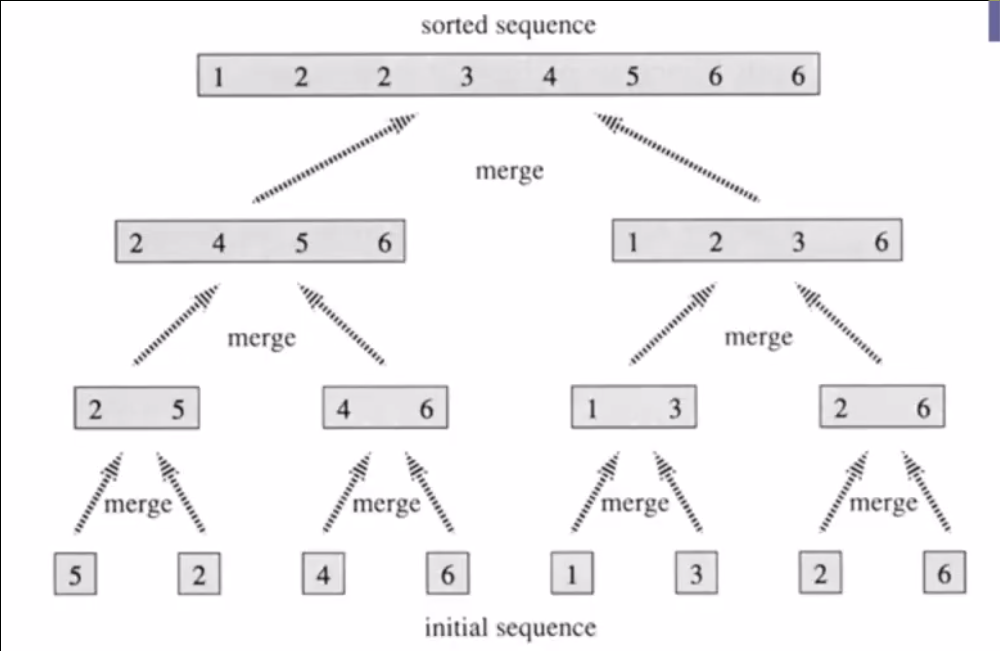
\includegraphics[keepaspectratio,width=0.4\textwidth]{./img/merge_sort.png}
\caption{\label{fig:merge_sort}Representación gráfica del algoritmo \emph{mergesort}}
\end{figure}

En el primer piso del arbol (de abajo hacia arriba), cada mezcla requiere dos
operaciones; en el cuarto piso cada mezcla cuesta cuatro operaciones, y en el
tercer piso la mezcla cuesta ocho. Si observamos de manera detenida, observamos
que en realidad en cada piso requerimos \emph{n} operaciones. En el primero, una
mezcla cuesta dos operaciones, y son 4 mezclas, esto es: \(n = 4 \cdot 2\); en el
segundo piso, son dos mezclas, que requiere cuatro operaciones, esto es:
\(n = 2 \cdot 4\) y en el tercer y último piso, se hace una sola mezcla que cuesta
ocho operaciones, esto es: \(n = 1 \cdot 8\).

De esto concluimos que cada piso requiere \emph{n} operaciones; la siguiente pregunta
que queda por resolver es: ¿cuántas divisiones se van a hacer al arreglo
inicial?. La respuesta, como ya se ha mencionado es \(\log_2(n)\), ya que el
logaritmo nos indica cuántas veces se puede dividir un número \emph{n} entre la base,
en este caso, dos, ya que en cada división dividimos el array a la mitad.

De todo esto observamos que el tiempo de ejecución del algoritmo \emph{mergesort} es
$$
O(n \log_2 n)
$$
\subsubsection{Tiempo cuadrático \(O(n^2)\)}
\label{sec:org089d79b}
El tiempo cuadrático \(O(n^2)\) crece de manera parabólica conforme
el tamaño de la entrada al algoritmo aumenta. Ejemplos de algoritmos con tiempo
cuadrático de ejecución son:
\begin{itemize}
\item Enumeración de todos los pares de elementos
\begin{itemize}
\item Emparejamiento estable
\item Simulación gravitatoria
\end{itemize}
\item Encontrar el par de puntos más cercano
\begin{itemize}
\item Dada una lista de puntos, encontrar los dos que se encuentran más cerca.
\end{itemize}
\end{itemize}
\subsubsection{Tiempo cúbico \(O(n^3)\)}
\label{sec:org2fa2070}
Estos algoritmos crecen como una función cúbica conforme su entrada aumenta. Por
ejemplo:
\begin{itemize}
\item Enumeración de todos los tríos de elementos
\item Determinar si \emph{n} conjuntos son disjuntos
\begin{itemize}
\item Dados \emph{n} conjuntos \(S_1, S_2, \cdots, S_n\) cada cual es subconjunto de
\(\{1, 2, \cdots, n\}\), determinar si existe algún par de conjuntos que
sean disjuntos.
\end{itemize}
\end{itemize}
\begin{verbatim}
for (each_set_Si)
{
    for(each_set_Sj)
    {
        for(each_element_p_of_Si)
            // determine whether p also belongs to Sj
    }
    if (no_element_of_Si_belongs_to_Sj)
        // report that Si and Sj are disjoint
}
\end{verbatim}
\subsubsection{Tiempo polinomial \(O(n^k)\)}
\label{sec:org1f033aa}
El tiempo polinomial es una generalización de los tiempos de ejecución cúbicos y
cuadráticos, donde \emph{k} representa una potencia positiva de \emph{n}. Ejemplos:
\begin{itemize}
\item Conjunto independiente
\begin{itemize}
\item ¿Dado un grafo, existen \emph{k} nodos tales que no están unidos por una
arista?
\item Solución de tiempo de \(O(n^k)\)
\end{itemize}
\end{itemize}
\end{document}
